\chapter{Task 3}
\begin{parlist}
	\item If actions are bounded to state transitions, their contents would be written onto the transition arrow, meaning that the activity that the arrow is depicting yields a state change. Whereas if the activity is depicted inside the state itself, means that no state change happens and/or the action itself gets activated when the the machine enters the state.
	\item Solution:
	\begin{figure}[hbt]
  \makebox[\textwidth][c]{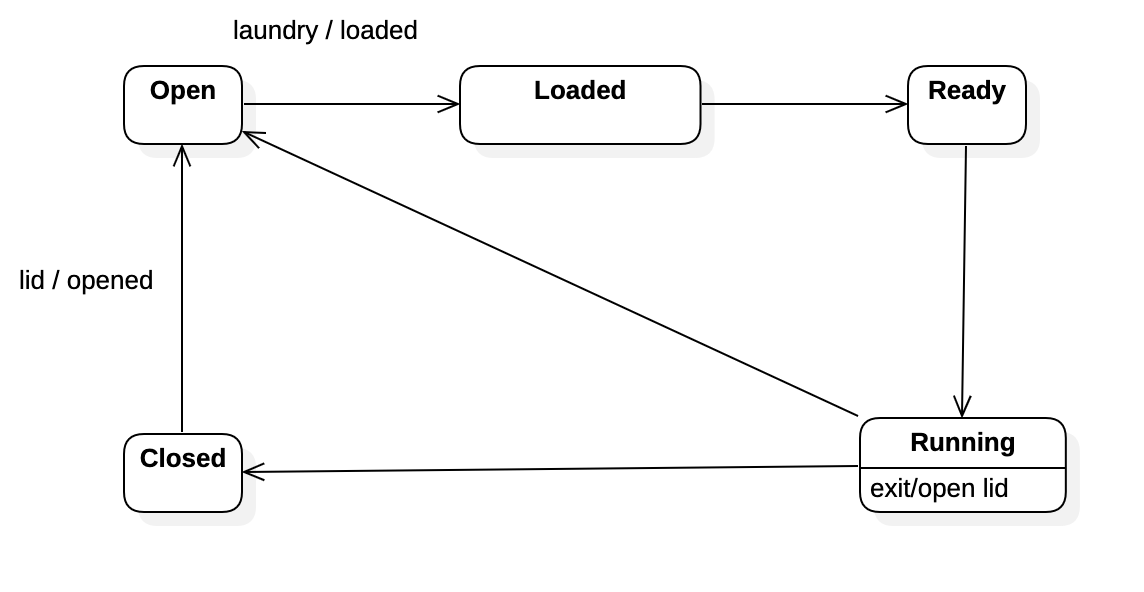
\includegraphics[width=1.5\textwidth]{Immagini/StatechartDiagram.png}}
  \caption{}
\end{figure}

\end{parlist}
